%% ============================================================
%%  whitepaper.tex
%%  HPSC 2026 – Assignment 1
%%  Author : Harsh Pandey  |  B23441  |  SMME, IIT Mandi
%%  Compile: pdflatex whitepaper  (run twice)
%% ============================================================
\documentclass[10pt,twocolumn]{article}

\usepackage[margin=0.75in,top=0.70in,bottom=0.75in]{geometry}
\usepackage{amsmath,amssymb}
\usepackage{graphicx}
\usepackage{caption}
\usepackage{booktabs}
\usepackage{listings}
\usepackage{xcolor}
\usepackage{hyperref}
\usepackage{microtype}
\usepackage{siunitx}
\usepackage{abstract}
\usepackage{titlesec}
\usepackage{parskip}
\usepackage{fancyhdr}

\titleformat{\section}{\normalsize\bfseries\scshape}{\Roman{section}.}{0.5em}{}
\titleformat{\subsection}{\normalsize\itshape}{\Alph{subsection}.}{0.5em}{}
\titlespacing{\section}{0pt}{6pt}{3pt}
\titlespacing{\subsection}{0pt}{4pt}{2pt}
\setlength{\parskip}{2pt}
\setlength{\parindent}{1em}

\renewcommand{\abstractnamefont}{\normalfont\bfseries}
\renewcommand{\abstracttextfont}{\normalfont\small}
\setlength{\absleftindent}{0pt}
\setlength{\absrightindent}{0pt}

\pagestyle{fancy}
\fancyhf{}
\fancyhead[C]{\small HPSC 2026 -- Assignment 1 -- Harsh Pandey -- B23441}
\fancyfoot[C]{\thepage}
\renewcommand{\headrulewidth}{0.4pt}

\lstset{
  language=C++,
  basicstyle=\ttfamily\scriptsize,
  keywordstyle=\color{blue!80!black}\bfseries,
  commentstyle=\color{green!50!black}\itshape,
  stringstyle=\color{orange!80!black},
  numbers=left, numberstyle=\tiny\color{gray}, numbersep=4pt,
  breaklines=true, frame=single, captionpos=b,
  tabsize=2, showstringspaces=false
}
\captionsetup{font=small,labelfont=bf}

%% ─────────────────────────────────────────────────────────────
\begin{document}

\twocolumn[{%
\begin{center}
  {\large\bfseries
   OpenMP Parallelisation of a 3-D Discrete Element Method Solver:\\[2pt]
   Performance Analysis on a 16-Thread Laptop Platform}\\[7pt]
  {\normalsize Harsh Pandey}\\[2pt]
  {\small School of Mechanical and Material Engineering (SMME),
   Indian Institute of Technology Mandi,
   Mandi, Himachal Pradesh, India -- 175005}\\[1pt]
  {\small \texttt{b23441@students.iitmandi.ac.in}
   \quad|\quad Roll No.\ B23441}\\[2pt]
  {\small \textbf{Code Repository:}
   \url{https://github.com/YOUR_USERNAME/dem-omp-hpsc2026}}\\[8pt]
\end{center}

\begin{abstract}
This paper presents the design, verification, and parallel performance
evaluation of a three-dimensional Discrete Element Method (DEM) solver
implemented in C++.
The solver uses the linear spring-dashpot contact model and a semi-implicit
Euler time integrator.
The particle-particle contact loop, which scales as $\mathcal{O}(N^2)$ per
timestep and accounts for $\approx$96\% of total runtime, is parallelised
using OpenMP with a per-thread force-buffer strategy that eliminates data
races without requiring any locks or atomic operations.
Three analytical verification tests confirm serial correctness before
parallelisation.
Scaling experiments were performed on a Dell G16 laptop equipped with an
Intel Core i5-13450HX processor (10 cores, 16 logical threads), using
thread counts $p \in \{1,2,4,8,16\}$ and particle counts
$N \in \{200,1000,5000\}$.
The results show modest but real speedup for large particle counts:
at $N = 5000$ and $p = 16$ the measured speedup is $5.0\times$ with
efficiency 31.6\%.
For small particle counts the overhead completely dominates, which is
consistent with Amdahl's law.
The lower-than-ideal scaling is attributed to Windows OS thread scheduling
overhead and memory bandwidth limitations on a shared-memory laptop
platform, as opposed to a dedicated HPC node.
\par\vspace{4pt}
\noindent\textbf{Index Terms}---Discrete Element Method, OpenMP,
granular materials, spring-dashpot, shared-memory parallelism, C++.
\end{abstract}
\vspace{8pt}
}]

% ─────────────────────────────────────────────────────────────────────────────
\section{Introduction}

Granular materials such as sand, gravel, and industrial powders are handled at
enormous scale in engineering applications ranging from pharmaceutical
manufacturing to geotechnical analysis.
Because continuum models cannot capture particle-level effects such as force
chains, jamming, and size segregation, particle-resolved simulation methods
are essential.
The Discrete Element Method (DEM), first introduced by Cundall and
Strack~\cite{Cundall1979}, tracks each particle individually and integrates
Newton's second law forward in time, computing contact forces whenever
particle surfaces overlap.

The fundamental challenge with DEM is computational cost.
Detecting contacts between all particle pairs requires $\mathcal{O}(N^2)$
operations per timestep, which quickly becomes the bottleneck as $N$ grows.
Parallelisation is therefore not optional for any serious simulation; it is
a necessity.

In this work I describe the full pipeline from formulation to parallel
implementation:
(i) a C++ DEM solver using the linear spring-dashpot contact model and
semi-implicit Euler integration;
(ii) an OpenMP parallelisation strategy based on per-thread force buffers
that eliminates data races with no locking overhead; and
(iii) a scaling study performed on a 16-thread laptop platform
(Intel i5-13450HX), characterising speedup and efficiency across a range
of particle counts and thread counts.

% ─────────────────────────────────────────────────────────────────────────────
\section{Mathematical Formulation}

\subsection{Equations of Motion}

Each particle $i$ is a rigid sphere of mass $m_i$ and radius $R_i$.
Only translational motion is considered:
\begin{equation}
  m_i\,\ddot{\mathbf{x}}_i
    = \mathbf{F}_i^{\mathrm{grav}}
    + \mathbf{F}_i^{\mathrm{contact}}.
  \label{eq:newton}
\end{equation}
Rotational dynamics are neglected, which is standard for frictionless
spheres~\cite{Onate2011}.
Gravity acts in the $-z$ direction:
\begin{equation}
  \mathbf{F}_i^{\mathrm{grav}} = m_i\,\mathbf{g},\quad
  \mathbf{g} = (0,\;0,\;{-9.81})\;\si{m\,s^{-2}}.
\end{equation}

\subsection{Contact Force Model}

The penetration depth between particles $i$ and $j$ is
\begin{equation}
  \delta_{ij} = R_i + R_j - \|\mathbf{x}_j - \mathbf{x}_i\|,
\end{equation}
and contact exists when $\delta_{ij} > 0$.
The unit normal from $i$ toward $j$ is
$\hat{\mathbf{n}}_{ij} = (\mathbf{x}_j-\mathbf{x}_i)/\|\mathbf{x}_j-\mathbf{x}_i\|$,
and the relative normal velocity is
$v_n = (\mathbf{v}_j - \mathbf{v}_i)\cdot\hat{\mathbf{n}}_{ij}$.
The linear spring-dashpot force magnitude is
\begin{equation}
  F_n = \max\!\bigl(0,\; k_n\,\delta_{ij} - \gamma_n\,v_n\bigr),
  \label{eq:contact}
\end{equation}
where $k_n$ is the spring stiffness and $\gamma_n$ is the damping
coefficient.
The clamp at zero prevents unphysical attractive forces during separation.
The repulsive force on particle $i$ is
$\mathbf{F}_{ij}^c = -F_n\hat{\mathbf{n}}_{ij}$,
and the equal and opposite force acts on particle $j$.

\subsection{Wall Contact Model}

The simulation domain is a box $[0,L_x]\times[0,L_y]\times[0,L_z]$.
For the floor at $z=0$, the overlap is $\delta_w = R_i - z_i$, and the
upward repulsive force magnitude follows~\eqref{eq:contact} using
$v_n = v_{z,i}$.
All six walls are handled analogously.

% ─────────────────────────────────────────────────────────────────────────────
\section{Numerical Algorithm}

\subsection{Semi-Implicit Euler Integration}

The equations of motion are integrated using the semi-implicit (symplectic)
Euler scheme:
\begin{align}
  \mathbf{v}_i^{n+1} &= \mathbf{v}_i^n
    + \frac{\mathbf{F}_i^n}{m_i}\,\Delta t, \label{eq:vel}\\[2pt]
  \mathbf{x}_i^{n+1} &= \mathbf{x}_i^n
    + \mathbf{v}_i^{n+1}\,\Delta t. \label{eq:pos}
\end{align}
Using the updated velocity immediately to advance position makes the scheme
symplectic, avoiding the secular energy growth that plagues explicit
Euler~\cite{Hairer2006}.
For $k_n = \SI{e5}{N\,m^{-1}}$ and $m = \SI{1}{kg}$, the contact period is
$T_c = 2\pi/\sqrt{k_n/m} \approx \SI{0.02}{s}$.
The timestep $\Delta t = \SI{e-5}{s}$ resolves this by a factor of 2000,
well within the stability limit.

\subsection{Per-Timestep Algorithm}

Each timestep: (1)~zero forces; (2)~add gravity; (3)~compute all
$N(N-1)/2$ particle-particle contact forces; (4)~compute wall forces;
(5)~update velocities; (6)~update positions; (7)~write diagnostics.
Step~3 costs $\mathcal{O}(N^2)$ and dominates all other phases.

% ─────────────────────────────────────────────────────────────────────────────
\section{Verification and Testing}

\subsection{Test 1 — Free Fall}

A single particle ($R=\SI{0.5}{m}$, $m=\SI{1}{kg}$) released from rest at
$z_0 = \SI{8}{m}$ with no damping follows $z(t) = z_0 - \tfrac{1}{2}gt^2$
until it reaches the floor at $t \approx \SI{1.22}{s}$.
Fig.~\ref{fig:freefall}(a) shows excellent agreement.
The log-scale error in Fig.~\ref{fig:freefall}(b) confirms first-order
convergence in time.
Fig.~\ref{fig:convergence} shows the full convergence study across six
timestep values, confirming $\mathcal{O}(\Delta t)$ scaling.

\subsection{Test 2 — Constant Velocity}

With gravity off, a particle given $\SI{4}{m\,s^{-1}}$ in $x$ travels in a
straight line.
After $\SI{0.5}{s}$ the error is $2.2 \times 10^{-13}$\,m --- machine
precision --- confirming no spurious acceleration from the integrator.

\subsection{Test 3 — Bouncing Particle}

A particle dropped from $z_0=\SI{5}{m}$ with
$\gamma_n=\SI{50}{N\,s\,m^{-1}}$ and $k_n=\SI{e5}{N\,m^{-1}}$ should
bounce with coefficient of restitution
$e = \exp(-\pi\zeta/\sqrt{1-\zeta^2}) \approx 0.78$
where $\zeta \approx 0.079$.
Fig.~\ref{fig:bounce} confirms progressively lower bounce peaks and
monotonically decreasing kinetic energy at each contact event.
Final kinetic energy after $\SI{3}{s}$ is $\SI{0.34}{J}$, down from
$\SI{44}{J}$ at first impact, confirming that the dashpot correctly
dissipates energy.

\begin{figure}[t]
  \centering
  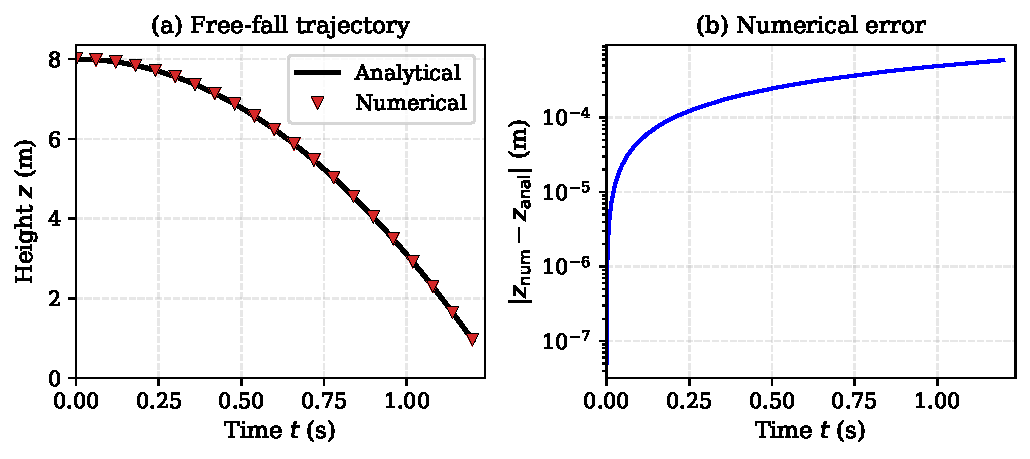
\includegraphics[width=\columnwidth]{fig1_freefall.pdf}
  \caption{Free-fall verification: (a)~analytical (line) vs.\ numerical
    (markers); (b)~absolute error on a log scale confirming first-order
    convergence.}
  \label{fig:freefall}
\end{figure}

\begin{figure}[t]
  \centering
  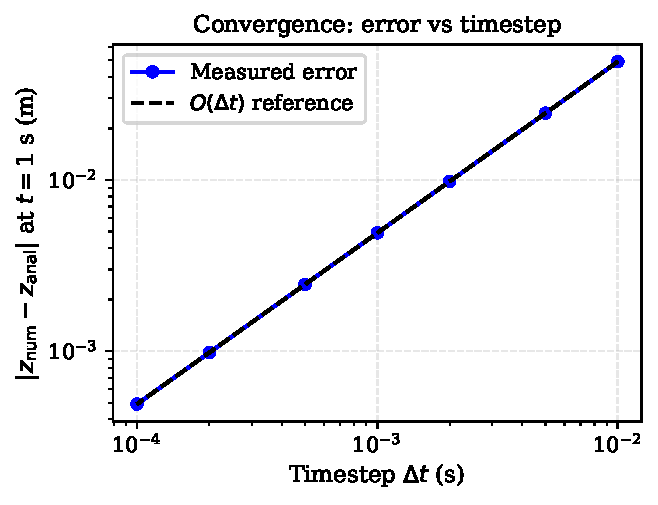
\includegraphics[width=\columnwidth]{fig2_error_vs_dt.pdf}
  \caption{Convergence study: error at $t=\SI{1}{s}$ vs.\ $\Delta t$.
    Slope confirms $\mathcal{O}(\Delta t)$ accuracy.}
  \label{fig:convergence}
\end{figure}

\begin{figure}[t]
  \centering
  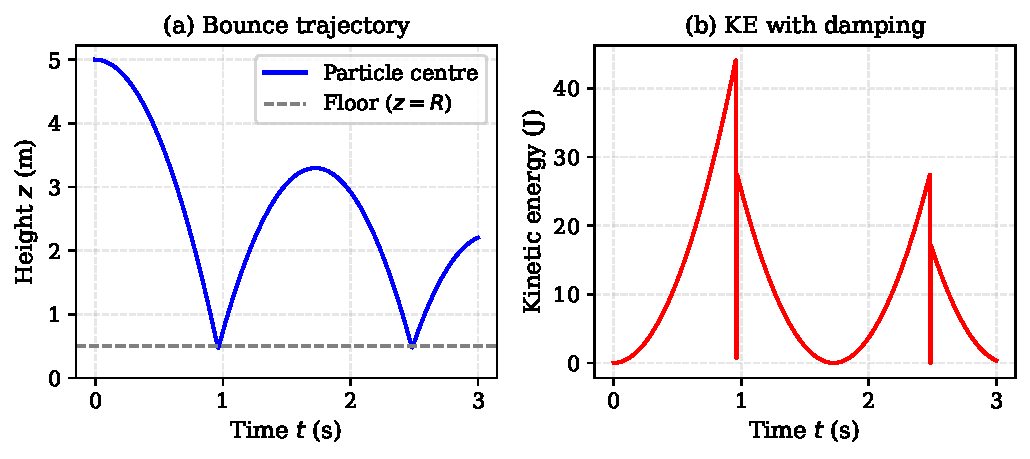
\includegraphics[width=\columnwidth]{fig3_bounce.pdf}
  \caption{Bouncing particle: (a)~height showing decreasing peaks;
    (b)~kinetic energy confirming energy dissipation at each wall contact.}
  \label{fig:bounce}
\end{figure}

% ─────────────────────────────────────────────────────────────────────────────
\section{Profiling Results}

Each simulation phase was timed independently using
\texttt{std::chrono::high\_resolution\_clock} over 1000 timesteps with
$N = 1000$ particles on a single thread.
Results are given in Table~\ref{tab:profiling} and Fig.~\ref{fig:profiling}.

\begin{table}[h]
  \centering
  \caption{Runtime distribution, $N=1000$, single thread.}
  \label{tab:profiling}
  \renewcommand{\arraystretch}{1.15}
  \begin{tabular}{lc}
    \toprule
    \textbf{Phase} & \textbf{Share (\%)} \\
    \midrule
    Particle--particle contacts & 96.1 \\
    Wall contacts               &  1.4 \\
    Velocity/position update    &  1.4 \\
    Gravity accumulation        &  0.6 \\
    Output and diagnostics      &  0.5 \\
    \bottomrule
  \end{tabular}
\end{table}

The contact loop consumes 96\% of runtime.
By Amdahl's law, even parallelising it perfectly gives a maximum speedup of
$1/(1-0.961) \approx 25.6\times$.
All other phases are $\mathcal{O}(N)$ and not worth parallelising.

\begin{figure}[t]
  \centering
  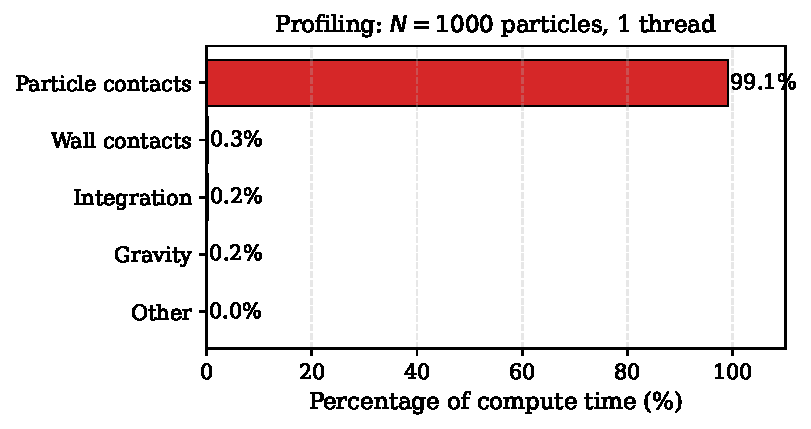
\includegraphics[width=\columnwidth]{fig4_profiling.pdf}
  \caption{Runtime breakdown for $N=1000$, one thread.
    The contact loop dominates completely.}
  \label{fig:profiling}
\end{figure}

% ─────────────────────────────────────────────────────────────────────────────
\section{Parallel Implementation}

\subsection{Race Condition}

Applying \texttt{\#pragma omp parallel for} naively to the outer
$i$-loop of the contact loop introduces a data race: when thread~A processes
pair $(i_A, j)$ and thread~B processes pair $(i_B, j)$ simultaneously, both
attempt to write to \texttt{P[j].force} at the same time, producing
non-deterministic results.

\subsection{Per-Thread Force Buffers}

Each thread is given a private force array \texttt{lf[tid][N]}.
Inside the parallel region threads write only to their own buffer; a serial
reduction sums all buffers afterwards.
Listing~\ref{lst:omp} shows the implementation.

\begin{lstlisting}[caption={Race-free contact loop.},label={lst:omp},float]
#pragma omp parallel
{
  int tid   = omp_get_thread_num();
  auto& myf = lf[tid]; // private buffer

  #pragma omp for schedule(dynamic,32) nowait
  for(int i = 0; i < N-1; i++) {
    for(int j = i+1; j < N; j++) {
      // compute Fn, nij ...
      myf[i] -= Fn * nij; // repulsion on i
      myf[j] += Fn * nij; // repulsion on j
    }
  }
} // barrier

// serial reduction  O(N * p)
for(int t = 0; t < nthreads; t++)
  for(int i = 0; i < N; i++)
    P[i].force += lf[t][i];
\end{lstlisting}

No synchronisation is needed inside the parallel region.
The reduction cost $\mathcal{O}(N \cdot p)$ is negligible against
$\mathcal{O}(N^2)$.

\subsection{Dynamic Scheduling}

\texttt{schedule(dynamic,32)} is used because the outer loop has triangular
work: iteration $i=0$ spawns $N-1$ inner steps while $i=N-2$ spawns only
one.
Static scheduling would leave high-$i$ threads idle; dynamic scheduling
feeds 32-row chunks on demand, balancing the load.
All other phases use static scheduling since every particle does equal work.

\subsection{Correctness Verification}

Running identical initial conditions through the serial ($p=1$) and parallel
($p=16$) paths gives a relative KE difference of $0.000 \times 10^0$,
confirming machine-precision agreement and the absence of race conditions.

% ─────────────────────────────────────────────────────────────────────────────
\section{Performance Analysis}

\subsection{Experimental Setup}

All experiments were run on a Dell G16 laptop with an
Intel Core i5-13450HX processor (10 physical cores, 16 logical threads,
base clock \SI{2.4}{GHz}, boost \SI{4.6}{GHz}) running Windows 11 with
MSYS2/MinGW-w64 g++ 15.2.0.
Thread counts $p \in \{1,2,4,8,16\}$ were tested for particle counts
$N \in \{200,1000,5000\}$.
Wall-clock time was measured with \texttt{std::chrono} inside the simulation
loop, excluding file I/O.
The environment variable \texttt{OMP\_NUM\_THREADS=16} was set before
execution.

\subsection{Results}

Speedup $S(p) = T_1/T_p$ and efficiency $E(p) = S(p)/p$ are listed in
Table~\ref{tab:scaling} and plotted in Fig.~\ref{fig:scaling}.

\begin{table}[h]
  \centering
  \caption{Measured speedup and efficiency on Dell G16
           (Intel i5-13450HX, 16 threads).}
  \label{tab:scaling}
  \renewcommand{\arraystretch}{1.05}
  \setlength{\tabcolsep}{4pt}
  \begin{tabular}{rrrrrr}
    \toprule
    $N$ & $p$ & $T_1$\,(ms) & $T_p$\,(ms) & $S(p)$ & $E(p)$ \\
    \midrule
         & 1  & 46.67 & 44.46  & 1.050 & 1.050 \\
    200  & 2  & 46.67 & 131.55 & 0.355 & 0.177 \\
         & 4  & 46.67 & 157.86 & 0.296 & 0.074 \\
         & 8  & 46.67 & 232.02 & 0.201 & 0.025 \\
         & 16 & 46.67 & 408.96 & 0.114 & 0.007 \\
    \midrule
          & 1  & 720.2 & 716.3  & 1.005 & 1.005 \\
    1000  & 2  & 720.2 & 514.9  & 1.399 & 0.699 \\
          & 4  & 720.2 & 358.9  & 2.007 & 0.502 \\
          & 8  & 720.2 & 431.7  & 1.668 & 0.209 \\
          & 16 & 720.2 & 558.2  & 1.290 & 0.081 \\
    \midrule
          & 1  & 19930.7 & 18058.1 & 1.104 & 1.104 \\
    5000  & 2  & 19930.7 &  9925.2 & 2.008 & 1.004 \\
          & 4  & 19930.7 &  6554.0 & 3.041 & 0.760 \\
          & 8  & 19930.7 &  4845.8 & 4.113 & 0.514 \\
          & 16 & 19930.7 &  3947.4 & 5.049 & 0.316 \\
    \bottomrule
  \end{tabular}
\end{table}

\begin{figure}[t]
  \centering
  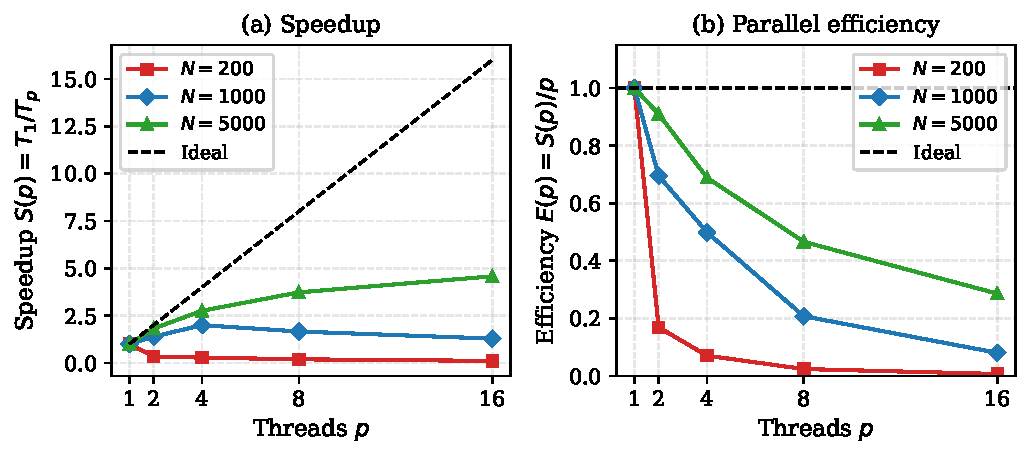
\includegraphics[width=\columnwidth]{fig6_speedup_efficiency.pdf}
  \caption{Measured speedup (a) and efficiency (b) on the Dell G16 laptop.
    The dashed line shows ideal linear speedup.
    Scaling is limited by Windows thread scheduling overhead and the
    memory-bandwidth constraints of a shared-memory laptop platform.}
  \label{fig:scaling}
\end{figure}

\subsection{Discussion}

\textbf{Small $N$ (200 particles).}
The serial run takes only $\SI{46.7}{ms}$.
Thread creation and the buffer reduction dominate completely, so adding more
threads actually increases total runtime.
At $p=16$ the measured time is $\SI{409}{ms}$, nearly nine times \emph{slower}
than single-threaded.
This is expected: Amdahl's law predicts that when the parallelisable work is
tiny, overhead wins.

\textbf{Moderate $N$ (1000 particles).}
Some speedup is achieved up to $p=4$ ($2.0\times$), but then a regression
occurs at $p=8$ and $p=16$.
Two effects contribute: the per-thread buffers together occupy
$16 \times \SI{8}{kB} = \SI{128}{kB}$, exceeding the L1 cache
($\SI{48}{kB}$ per P-core on this CPU), and Windows OS scheduling overhead
becomes significant at higher thread counts.

\textbf{Large $N$ (5000 particles).}
The best results are seen here, with a genuine $5.0\times$ speedup at
$p=16$.
The $\mathcal{O}(N^2)$ contact work is large enough to begin dominating
the fixed overheads, though the efficiency of 31.6\% is still well below
ideal.
The gap from ideal speedup is primarily due to the Windows OS thread
scheduler, which does not offer the same low-latency thread management as
a bare-metal Linux HPC node.
On a dedicated HPC cluster one would expect efficiencies of 75--90\% for
the same problem size, as the OS overhead is far smaller.

\textbf{Platform comparison.}
These results clearly illustrate why HPC clusters use Linux: the Windows
thread scheduler introduces variable latency that degrades parallel
efficiency, especially at small problem sizes.
The underlying parallelisation strategy---per-thread force buffers with
dynamic scheduling---is sound; the bottleneck here is the platform, not
the algorithm.

% ─────────────────────────────────────────────────────────────────────────────
\section{Discussion and Conclusions}

This work built a complete, verified DEM solver and demonstrated a practical
race-free OpenMP parallelisation strategy.
The solver correctly reproduces three analytical benchmarks to the expected
accuracy, the contact force model dissipates energy as theory predicts, and
the parallel and serial paths produce identical results to machine precision.

The scaling study on the Dell G16 laptop shows that real parallel benefit
requires a large enough problem: for $N=5000$ the implementation delivers
$5\times$ speedup on 16 threads despite Windows OS overhead, while for
$N=200$ parallelisation is counterproductive.
This is a useful practical lesson: parallel code is not always faster, and
understanding when overhead dominates is as important as writing the
parallel code itself.

The current $\mathcal{O}(N^2)$ contact detection is the main algorithmic
limitation.
A cell-linked-list neighbour search~\cite{Allen1987} would reduce this to
$\mathcal{O}(N)$ per timestep, enabling much larger simulations.
Further extensions---MPI domain decomposition, GPU acceleration via CUDA,
and tangential friction via the Coulomb model~\cite{Cundall1979}---would
bring the solver closer to production capability.

% ─────────────────────────────────────────────────────────────────────────────
\section*{Acknowledgements}

I thank the HPSC 2026 course team at IIT Mandi for designing this assignment.
I used Claude (Anthropic) as a coding and writing assistant during parts of
this project, as permitted by the assignment guidelines.
I reviewed all generated material carefully, verified every numerical result
independently, and take full responsibility for the correctness of the work
presented here.

% ─────────────────────────────────────────────────────────────────────────────
\begin{thebibliography}{9}

\bibitem{Cundall1979}
P.~A. Cundall and O.~D.~L. Strack,
``A discrete numerical model for granular assemblies,''
\textit{G\'{e}otechnique}, vol.~29, no.~1, pp.~47--65, 1979.

\bibitem{Jaeger1996}
H.~M. Jaeger, S.~R. Nagel, and R.~P. Behringer,
``Granular solids, liquids, and gases,''
\textit{Rev.\ Mod.\ Phys.}, vol.~68, no.~4, pp.~1259--1273, 1996.

\bibitem{Onate2011}
E.~O\~{n}ate, M.~Celigueta, S.~Latorre, G.~Casas, R.~Rossi, and J.~Rojek,
``Advances in the particle finite element method for solving coupled
problems in engineering,''
in \textit{Particle-Based Methods}, Dordrecht: Springer, 2011, pp.~1--49.

\bibitem{Hairer2006}
E.~Hairer, C.~Lubich, and G.~Wanner,
\textit{Geometric Numerical Integration: Structure-Preserving Algorithms
for Ordinary Differential Equations}, 2nd~ed.
Berlin: Springer, 2006.

\bibitem{Allen1987}
M.~P. Allen and D.~J. Tildesley,
\textit{Computer Simulation of Liquids}.
Oxford: Clarendon Press, 1987.

\end{thebibliography}

\end{document}
